\documentclass{report}

%Packages pour les langues
\usepackage[utf8]{inputenc}
\usepackage[T1]{fontenc}
\usepackage[french]{babel}
\usepackage{lmodern}

%Package pour la mise en forme (marges)
\usepackage[a4paper]{geometry}
\geometry{hscale=0.85,vscale=0.85,centering}
\usepackage{layouts} %affichage des largeurs de zone texte
\usepackage{parallel}
\usepackage{setspace}
\usepackage{wrapfig}
%Packages pour les liens dynamiques
%\usepackage{hyperref}

%Packages pour les formules de Maths
\usepackage{amsmath}
\usepackage{amssymb}
\usepackage{mathrsfs}

%Packages des images
\usepackage{graphicx}

%\usepackage{subfigure}
\usepackage{subfig}
\usepackage{wrapfig}
\usepackage{caption}

%\usepackage{subcaption}
\usepackage{float}

%Packages pour le glossaire
\usepackage{glossaries}

%\usepackage[xindy]{glossaries}
\makeglossaries

%Package pour colorier le code Matlab (copyright Jérémy Fauvel)
\usepackage{listings}
\usepackage[usenames,dvipsnames]{color}

%Code pour afficher du code Matlab
\definecolor{MyDarkGreen}{rgb}{0.0,0.4,0.0}
\lstset{language=Matlab, frame=none, basicstyle=\small\ttfamily, keywordstyle=[1]\color{Blue}\bfseries, keywordstyle=[2]\color{Purple}, keywordstyle=[3]\color{Blue}\underbar, identifierstyle=, commentstyle=\usefont{T1}{pcr}{m}{sl}\color{MyDarkGreen}\small, stringstyle=\color{Purple}, showstringspaces=false, tabsize=5, morekeywords={xlim,ylim,var,alpha,factorial,poissrnd,normpdf,normcdf}, morekeywords=[2]{on, off, interp}, morekeywords=[3]{FindESS, homework_example}, morecomment=[l][\color{Blue}]{...}, numbers=left, firstnumber=1, numberstyle=\tiny\color{Red}, stepnumber=1}

%Packages pour les string
\usepackage{xstring}

%Packages pour les listes
%\usepackage{enumitem}

\begin{document}
\begin{titlepage}
\title{Rapport de stage - IRR \\ Implémentation et application d'un algorithme dynamique hybride pour le contrôle d'articulations flexibles}
\date{3 Mars 2014 - 31 Août 2014}
\author{Auteur: \bsc{Guedelha} Nuno \\ Tuteur: \bsc{Stasse} Olivier}
\end{titlepage}



\graphicspath{{illustrations/}}
\maketitle

%Rennomer la table des matières en Sommaire
\renewcommand{\contentsname}{Sommaire}
\tableofcontents
\listoffigures
\listoftables

%%%%%%%%%%%%%%%%%% Macros %%%%%%%%%%%%%%%%%%%%%%%%%%%%%%%

%=============== variable fichier de figures ==============================

\newcommand{\myFiguresFile}{}
\newcommand{\setmyFiguresFile}[1]{\renewcommand{\myFiguresFile}{#1}}

%=============== include 1 figure =========================================

\ifx \incFig \undefined
\def \incFig [#1]#2{\includegraphics[width=#2, page=#1]{figs/\myFiguresFile}}
\fi

%=============== Display 1 figure =========================================

\ifx \dispFig \undefined
\def \dispFig [#1]#2#3#4#5%
{
\begin{figure}[#1]
  \begin{center}
  \includegraphics[width=#3, page=#2]{figs/\myFiguresFile}
  \IfStrEq{#4}{}{}{%
    \caption{#4}  % legende
    \label{#5}    % pour citer le numéro de figure
  }
  \end{center}
\end{figure}
}
\fi

%=============== 2 sous-figures alignées horizontalement =================

\ifx \dispTwoFig \undefined
\def \dispTwoFig [#1]#2#3#4#5#6#7%
{
\begin{figure}[#1]
\begin{center}
  \subfloat[#3 \label{#7.a}]{\includegraphics[width=7cm, page=#2]{figs/\myFiguresFile}}\hspace{1cm}
  \subfloat[#5 \label{#7.b}]{\includegraphics[width=7cm, page=#4]{figs/\myFiguresFile}}\hspace{1cm}
  \caption{#6}  % legende \\
  \label{#7} % pour citer le numéro de figure
\end{center}
\end{figure}
}
\fi

%=============== 3 sous-figures alignées horizontalement =================

\ifx \dispThreeFig \undefined
\def \dispThreeFig [#1]#2#3#4#5#6#7#8#9%
{
\begin{figure}[#1]
\begin{center}
  \subfloat[#3 \label{#9.a}]{\includegraphics[width=5cm, page=#2]{figs/\myFiguresFile}}\hspace{1cm}
  \subfloat[#5 \label{#9.b}]{\includegraphics[width=5cm, page=#4]{figs/\myFiguresFile}}\hspace{1cm}
  \subfloat[#7 \label{#9.c}]{\includegraphics[width=5cm, page=#6]{figs/\myFiguresFile}}\\
  \caption{#8}  % legende
  \label{#9}    % pour citer le numéro de figure
\end{center}
\end{figure}
}
\fi

%=============== 2 ou 3 colonnes alignée horizontalement ==================

\ifx \minipages \undefined
\def \minipages [#1]#2#3#4#5#6#7#8%
{
\begin{minipage}[#2]{#3\textwidth}
  #6
\end{minipage}
\begin{minipage}[#2]{#4\textwidth} \hfill
  #7
\end{minipage}
\IfStrEq{#1}{3}%
{
\begin{minipage}[#2]{#5\textwidth} \hfill
  #8
\end{minipage}
}
}
\fi

%=============== exemples ==================================================

%\begin{minipage}{.3\textwidth} \hfill
%  \begin{align*}
%  D_{O} = \lbrace &\textbf{d}_{Ox}, \textbf{d}_{Oy}, \textbf{d}_{Oy}, \\
%  &\textbf{d}_{x}, \textbf{d}_{y}, \textbf{d}_{z} \rbrace \subset M^{6}
%  \end{align*}
%\end{minipage}
%\begin{minipage}{.4\textwidth} \hfill
%  \begin{tabbing}
%  \= $\textbf{d}_{Ox}$ \= vecteur unitaire de rotation autour de $O_{x}$\\
%  \> $\textbf{d}_{Oy}$ \> vecteur unitaire de rotation autour de $O_{y}$\\
%  \> $\textbf{d}_{Oz}$ \> vecteur unitaire de rotation autour de $O_{z}$\\
%  \> $\textbf{d}_{x}$  \> vecteur unitaire de translation le long de $O_{x}$\\
%  \> $\textbf{d}_{y}$  \> vecteur unitaire de translation le long de $O_{y}$\\
%  \> $\textbf{d}_{z}$  \> vecteur unitaire de translation le long de $O_{z}$\\
%  \end{tabbing}
%\end{minipage}

%=============== autres macro textuelles ===================================

\newcommand{\cad}[0]{\textnormal{c'est à dire }}

\newcommand{\valTextwidth}[0]{\thetextwidth}

\newcommand{\valTextwidthUnit}[1]{\printinunitsof{#1}\prntlen{\textwidth}}

\newcommand{\valInUnit}[2]{\printinunitsof{#1}\prntlen{#2}}

%affichage des largeurs de zone texte
%\usepackage{layouts}
%\printinunitsof{cm}\prntlen{\textwidth}

\newcommand{\newglossdef}[3]
{\newglossaryentry{#1}%
{%
  name={#2},%
  description={#3}%
}}



%%%%%%%%%%%%%%%%%%%%%%%%%%%%%%%%%%%%%%%%%%%%%%%%%%%%%%%%%
\chapter*{Remerciements}
\addcontentsline{toc}{chapter}{Remerciements}

Je voudrais remercier, avant tout, tous ceux qui ont rendu cette expérience possible, et très enrichissante.\\
Je tiens à remercier dans un premier temps, toute l’équipe pédagogique du Master I.R.R. et les intervenants professionnels responsables de la formation, pour avoir assuré la partie académique de celle-ci. Je remercie Mme. Viviane Cadenat et M. Michel Taix pour leurs conseils sur les critères de choix d'une formation de 2ème cycle en Robotique, qui ont facilité mon orientation à l'origine de mon inscription en Master I.R.R.\\
Je remercie également Monsieur Vincent Durola, mon tuteur pédagogique attitré, pour ses conseils concernant la mission de ce stage, conseils qui m'ont permis de prendre du recul par rapport à mes tâches et aux différents aspects techniques.\\
Je tiens à remercier tout particulièrement et à témoigner toute ma reconnaissance aux membres de l'équipe Gepetto, pour l’expérience enrichissante qu’elles m’ont permis de vivre durant ces six mois au sein du LAAS :\\
Monsieur Olivier Stasse, pour m’avoir intégré rapidement au sein du laboratoire et m’avoir accordé toute sa confiance ; pour le temps qu’elle m’a consacré tout au long de cette période, sachant répondre à toutes mes interrogations ; sans oublier sa participation au cheminement de ce rapport.\\
Monsieur Jean Paul Laumond, Maximilien Naveau, Justin Carpentier, ainsi que l’ensemble des membres de l'équipe Gepetto pour leur accueil sympathique et leur coopération professionnelle tout au long de ces six mois.\\
Tous ceux qui ont délivré des formations techniques sur la planification de mouvements, la dynamique inverse et les algorithmes de contrôle.\\

\vspace{0.3cm} % retour à la ligne


%%%%%%%%%%%%%%%%%% glossaire %%%%%%%%%%%%%%%%%%%%%%%%%%%%


% acronymes

\newacronym{rneaLabel}{RNEA}{Recursive Newton-Euler Algorithm}
\newacronym{crbaLabel}{CRBA}{Composite Rigid Body Algorithm}
\newacronym{abaLabel}{ABA}{Articulated Body Algorithm}

%% définitions

\newglossdef{vecteurLie}
{vecteur lié}
{Un vecteur lié $(A,\textbf{V})$ est l'ensemble d'un point $A$ et d'un vecteur $\textbf{V}$ associé à $A$. Par exemple une force ou une vitesse appliquées à un point fixe d'un solide.}

\newglossdef{champVecteurs}
{champ de vecteurs}
{On appelle champ de vecteurs l'application qui fait correspondre, à tout point $A$ de \varepsilon, un vecteur $U$ d'un espace vectoriel $F$ de même dimension que \varepsilon. Par exemple les champs électrique $E$ et magnétique $B$ liés à une charge électrique \cite{bib_champVecteurs}.}

\newglossdef{champAntiSym}
{champ antisymétrique}
{Un champ de vecteurs est \emph{antisymétrique} s'il existe un vecteur $S$ tel que, quels que soient les points $A$ et $B$, on ait: $M(A)=M(B)+AB \times S$. Le vecteur $S$ est \emph{le vecteur} du champ antisymétrique \cite{bib_champVecteurs}.}

\newglossdef{torseur}
{torseur}
{un outil mathématique utilisé principalement en mécanique du solide, pour décrire leurs mouvements et les actions mécaniques qu'ils subissent. Un \emph{torseur} $[T]$ est l'ensemble d'un champ antisymétrique $M(A)$ et de son vecteur $S$. $M(A)$ et $S$ sont appelés respectivement \emph{moment} et \emph{vecteur} du torseur $[T]$.}


\glsaddall
\printglossary

%%%%%%%%%%%%%%%%%%%%%%%%%%%%%%%%%%%%%%%%%%%%%%%%%%%%%%%%%

\chapter*{Introduction}
\addcontentsline{toc}{chapter}{Introduction}

\section*{contexte}


\section*{problème posé et objectifs}


\section*{étude bibliographique}


\section*{annonce du plan}


%%%%%%%%%%%%%%%%%%%%%%%%%%%%%%%%%%%%%%%%%%%%%%%%%%%%%%%%%
\chapter{Concepts généraux sur le contrôle dynamique des robots totalement actionnés}

\section{généralités sur le contrôle en couple ou position (vitesse ou accélération), et cas d'utilisation}

\section{dynamique directe / inverse et cas d'utilisation}

dynamique directe => simulation
\vspace{0.3cm}

dynamique inverse => contrôle en couple
\vspace{0.3cm}

dynamique hybride => contrôle en couple, avec articulations spéciales:
\vspace{0.3cm}

	- articulation Freeflyer à la base du robot

	- articulation flexible	ou contraintes de force sur la trajectoire de l'outil terminal
	
	- usinage (force appliquée le long d'une trajectoire
	
	- manipulation de pièces
	
	- simplification d'une simulation de système en supprimant les articulations au contrôle parfait (couple adaptatif permettant d'asservir la position/vitesse/accélération)


\section{contrôle d'un robot humanoïde: modèle du double pendule inversé}

modèle du double pendule innversé

filtre de Kallmann

cinématique inverse vers l'espace des configurations

dynamique inverse dans l'espace des configurations

Problème de la flexibilité de la semelle du pied de HRP2

Asservissement du couple "Backdrive" appliqué de la cheville au sol

Application à la stabilisation du robot (Shuuji Kajita)

=> algorithme dynamique hybride nécessaire.

\section{implémentation et contraintes}
- performances: précision, vitesse d'exécution , taille du code\vspace{0.3cm}
- interface (vecteurs d'entrée / sortie)\vspace{0.3cm}
- langage de programmation\vspace{0.3cm}
- Algorithme générique pour tous les modèles URDF de robots (arbre cinématique), mais optimisé pour chaque modèle spécifique (template et meta-programing)\vspace{0.3cm}



%%%%%%%%%%%%%%%%%%%%%%%%%%%%%%%%%%%%%%%%%%%%%%%%%%%%%%%%%
\chapter{algèbre spatiale selon Roy Featherstone}
%Formalisme compacte et plus adapté :\vspace{0.3cm}
%- au calcul numérique et récursif\vspace{0.3cm}
%- au parcours en profondeur d'abord d'arbres cinématiques\vspace{0.3cm}

\setmyFiguresFile{figures}

L'algorithme de dynamique hybride a été implémenté suivant le formalisme présenté par Featherstone dans son ouvrage \cite{Featherstone} regroupant l'ensemble des algorithmes sur la dynamique des corps rigides: l'algorithme récursif de Newton-Euler (\emph{\gls{acr_rneaLabel}}), l'algorithme "corps rigide composite" (\emph{\gls{acr_crbaLabel}}) et l'algorithme de corps articulés (\emph{\gls{acr_abaLabel}}). Ce formalisme est basé sur l'algèbre spatiale, qui définit les grandeurs dynamiques à l'aide d'une notation condensée et efficace, et utilise très souvent des mécanismes récursifs comme le parcours en profondeur de graphes représentant l'arbre cinématique d'un robot. Nous allons présenter dans cette section les fondements de l'algèbre spatiale, ainsi que les algorithmes impliqués dans la construction de l'algorithme hybride: le \gls{acr_rneaLabel} et le \gls{acr_crbaLabel}.\\


\section{Algèbre spatiale: définition des vecteurs spatiaux et d'un modèle de système}

L'algèbre spatiale est un système de notation très concis et léger pour décrire la vitesse, l'accélération et les forces appliquées à des corps rigides, à l'aide de vecteurs à six dimensions (tenseurs) dits vecteurs spatiaux. Cette notation réduit grandement la taille des équations de mouvement des modèles cinématique et dynamique du robot. En particulier, elle simplifie la transformation des tenseurs entre les repères liés aux différents corps du robot. Quelques exemples seront donnés après la présentation de ces fondements.\\


\subsection{Vecteurs spatiaux: espaces mathématique et bases}

Pour décrire le mouvement d'un corps rigide dans un espace 3D, et ayant six degrés de liberté, nous devons décrire le déplacement en translation et en rotation. Pour cela, on définit des tenseurs combinant ces deux types de grandeurs dans des espaces de vecteurs à six dimensions (6D). On définit ainsi :\\
\begin{itemize}
\item dans un espace noté $M^{6}$, un tenseur de mouvement pour les vitesses ou accélérations du corps
\item dans l'espace noté $F^{6}$, un tenseur de forces pour les forces et les couples appliqués à ce même corps
\end{itemize}
On définit des bases dans ces espaces, ainsi que les opérateurs : somme, produit scalaire, produit vectoriel.\\
Le vecteur de coordonnée $\underline{m}=[m_{1},...,m_{6}]^T$ représente le vecteur $m$ dans la base ${d_{1},...,d_{6}}$ dans $M^{6}$.
De même, $\underline{f}=[f_{1},...,f_{6}]^T$ représente le vecteur $f$ dans la base ${e_{1},...,e_{6}}$ dans $F^{6}$.
Ces bases sont réciproques, normales :

$$
d_{i}\cdot e_{j}=
\begin{cases}
0 \colon i \neq j\\
1 \colon i = j
\end{cases}
$$

Ainsi le produit scalaire entre ces vecteurs s'exprime:

$$
"\cdot" : M^{6} \times D^{6} \mapsto R
\qquad
\qquad
m \cdot f = \underline{m}^T f
$$

\subsection{Vitesse}\label{ch_algSpa_Vitesse}

On veut exprimer la vitesse d'un corps solide dans l'espace $M^{6}$. On considère un corps en rotation autour d'un axe passant par un point $P$ du solide, avec une vitesse angulaire $w$, et en translation avec une vitesse linéaire $v_{P}$. On défini un repère $R_{O}$ dans l'espace à trois dimensions du solide ($R(O,x,y,z)$).

\dispTwoFig[H]
{1}{Rotation autour d'un point du solide $P$}
{2}{Rotation autour du centre du repère $O$}
{Vitesse d'un objet en mouvement quelconque (translation et rotation simultanées). Un nouveau point de vue pour le vecteur spatial.}
{fig_VitessePointCoincidant}


Soit $P'$ un point quelconque lié au corps solide $C$ (donc fixe dans n'importe quel repère lié au solide). La vitesse du point $P'$ dans $R$ est donnée par	$v_{P'}=v_{P}+\overrightarrow{P'P} \times w$ .\\
On imagine que le solide s'étend maintenant à tout l'espace autour de lui, englobant ainsi le repère $R$. On peut considérer ainsi un champ de vitesses associé au champ de position de tous les points du solide étendu. Soit le point de ce champ coïncidant avec le centre su repère $O$, autrement dit le point lié au solide (étendu) coïncidant avec $O$ au moment où on mesure la vitesse du solide. Soit $v_{O}$ la vitesse du solide en ce point. Il est impératif de remarquer que ce vecteur vitesse n'est pas lié au solide, mais plutôt au point fixe $O$ (voir l'annexe \ref{appx_torseursToalgSpa_torseurs_appl} sur les torseurs). Comme pour le point $P'$ évoqué précedemment, on a:
$$
v_{O} = v_{P} + w \times \overrightarrow{PO}\\
\Leftrightarrow v_{P} = v_{O} - w \times \overrightarrow{PO} = v_{O} + w \times \overrightarrow{OP}
$$

On peut donc voir le corps $C$ comme un solide en translation à la vitesse $v_{O}$ et en rotation autour d'un axe passant par $O$ (parallèle à l'axe défini initialement) à la vitesse angulaire $w$. La vitesse de tout point $P$ de ce solide dans le repère $R(O,x,y,z)$ est alors donnée par:
\begin{equation}
v_{P} = v_{O} + w \times \overrightarrow{OP}
\quad\quad
\footnote{Bien que la vitesse $v_{P}$ soit définie en fonction de $O$, elle ne dépend pas de l'origine choisie puisqu'il s'agit du vecteur vitesse associé à $P$ par le champ de vitesses du solide, qui lui est indépendant de l'origine. En effet, $v_{O}$ et $\overrightarrow{OP}$ dépendent tous deux de $O$, mais ces dépendances se compensent.}
\end{equation}

On veut exprimer les coordonnées de $w$ et $v_{O}$ dans le repère cartésien $R(O,x,y,z)$. Pour cela, on définit la base orthonormée de \emph{Plücker} dans l'espace des tenseurs de mouvement $M^{6}$:\\

\begin{figure}[H]
\minipages[3]{t}{.3}{.3}{.4}
{%
  \dispFig[H]{3}{4cm}{}{}
}{%
  \begin{align*}
  D_{O} = \lbrace &\textbf{d}_{Ox}, \textbf{d}_{Oy}, \textbf{d}_{Oy}, \\
  &\textbf{d}_{x}, \textbf{d}_{y}, \textbf{d}_{z} \rbrace \subset M^{6}
  \end{align*}
}{%
  \begin{tabbing}
  \= $\textbf{d}_{Ox}$ \= vecteur unitaire de rotation autour de $O_{x}$\\
  \> $\textbf{d}_{Oy}$ \> vecteur unitaire de rotation autour de $O_{y}$\\
  \> $\textbf{d}_{Oz}$ \> vecteur unitaire de rotation autour de $O_{z}$\\
  \> $\textbf{d}_{x}$  \> vecteur unitaire de translation le long de $O_{x}$\\
  \> $\textbf{d}_{y}$  \> vecteur unitaire de translation le long de $O_{y}$\\
  \> $\textbf{d}_{z}$  \> vecteur unitaire de translation le long de $O_{z}$\\
  \end{tabbing}
}
\caption{Base de \emph{Plücker} dans $M^{6}$}
\label{fig_basePlucker}
\end{figure}

Voici les coordonnées cartésiennes de $w$ et $v_{O}$, ainsi que leur concaténation constituant les coordonnées du vecteur spatial $\widehat{v}$ dans la base de \emph{Plücker}:\\

\begin{minipage}[c]{.55\textwidth}
$$
\underline{w}=
\begin{bmatrix}
w_{x} \\
w_{y} \\
w_{z}
\end{bmatrix}
\quad \texttt{et} \quad
\underline{v}_{O}=
\begin{bmatrix}
v_{Ox} \\
v_{Oy} \\
v_{Oz}
\end{bmatrix}
\quad \Rightarrow \quad
\underline{\widehat{v}}_{O}=
\begin{bmatrix}
\underline{w} \\
\underline{v}_{O}
\end{bmatrix}
=
\begin{bmatrix}
w_{x} \\
w_{y} \\
w_{z} \\
v_{Ox} \\
v_{Oy} \\
v_{Oz}
\end{bmatrix}
$$
\end{minipage}
\begin{minipage}[c]{.45\textwidth}
\begin{align*}
\quad \texttt{représentant} \quad
\widehat{v} = 
  &w_{x}\textbf{d}_{Ox} + w_{y}\textbf{d}_{Oy} + w_{z}\textbf{d}_{Oz} \\
  &+ v_{Ox}\textbf{d}_{x} + v_{Oy}\textbf{d}_{y} + v_{Oz}\textbf{d}_{z}
\end{align*}
\end{minipage}

\vspace{0.3cm} % retour à la ligne

Le vecteur spatial $\widehat{v}$ rassemble les six composantes représentant complètement les mouvements $\underline{w}$ et $\underline{v}_{O}$ du corps $C$. Ce vecteur a une propriété majeure qui est l'invariance par rapport à la base de \emph{Plücker} choisie. Si on définit deux bases de \emph{Plücker} différentes $D_{O}$ et $D_{P}$, centrées respectivement sur $O$ et $P$, ainsi que les vecteurs spatiaux associés $\widehat{v}$ et $\widehat{v'}$, on obtient:

\begin{align}
\widehat{v}  &= \underline{v}_{O} \cdot D_{O} \notag \\
\widehat{v'} &= \underline{v}_{P} \cdot D_{P} \notag \\
^{D_{O}}\widehat{v} \quad &= \quad ^{D_{O}}\widehat{v'}
\label{equ_invariant}
\end{align}


Les projections de ces deux vecteurs spatiaux $\widehat{v}$ et $\widehat{v'}$ dans la même base de \emph{Plücker} sont identiques \eqref{equ_invariant}. Il faut noter que si les deux bases ont la même orientation, elles auront les mêmes vecteurs unitaires de translation ($\textbf{d}_{x}$, $\textbf{d}_{y}$ et $\textbf{d}_{z}$), mais les vecteurs unitaires de rotations diffèrent si $O \neq P$ ne sont pas confondus, comme illustré dans le l'exemple de cas simple ci-dessous:

\begin{figure}[H]
\begin{center}
  \subfloat[Equivalence des vecteurs de translation.]{\includegraphics[width=.3\textwidth, page=4]{figs/figures}}\hspace{.05\textwidth}
  \subfloat[Visualisation de $\textbf{d}_{Py}$ et $\textbf{d}_{Pz}$ en $O$.]{\includegraphics[width=.3\textwidth, page=5]{figs/figures}}\hspace{.05\textwidth}
  \subfloat[Expression des vecteurs de rotation dans $D_{O}$]
  {%
  \begin{minipage}[t]{.2\textwidth}
  \begin{center}
    \(\begin{aligned}
      \textbf{d}_{Px} &= \textbf{d}_{Ox} \\
      \textbf{d}_{Py} &= \textbf{d}_{Oy}+r \textbf{d}_{z} \\
      \textbf{d}_{Pz} &= \textbf{d}_{Px}-r \textbf{d}_{y}
    \end{aligned}\)
  \end{center}
  \end{minipage}
  }
  \caption{Transformation des vecteurs unitaires de mouvement entre deux bases de \emph{Plücker} de même orientation}  % legende
  \label{fig_transPlucker}    % pour citer le numéro de figure
\end{center}
\end{figure}

Pour rapidement comprendre ces transformations, on peut visualiser un corps tournant autour de l'axe $P_{y}$ à la vitesse $w_{y}$. On définit initialement le vecteur spatial $\widehat{v'}$ en $P$ (\cad considérant l'axe de rotation du corps autour de $P_{y}$) est alors $w_{y}\textbf{d}_{Py}$. Or la vitesse d'un point lié au corps et passant par $O$ (par rapport au repère fixe $R(O,x,y,z)$) vaut $rw_{y}\textbf{d}_{z}$. Le vecteur spatial en $O$ (\cad considérant le corps en rotation autour de l'axe $O_{y}$) est alors $\widehat{v}=\textbf{d}_{Oy}+r\textbf{d}_{z}$.

La propriété d'invariance se vérifie pour tout point $O$ et $P$ fixes dans l'espace et une orientation quelconque des repères $R(O,x,y,z)$ et $R'(P,x,y,z)$. Nous pouvons trouver la démonstration complète de cette propriété d'invariance dans l'annexe \ref{appx_dem}.


\subsection{Force}

Nous nous intéressons à présent aux forces appliquées au corps rigide $\emph{C}$. Soit une force $\textbf{f}$ quelconque appliquée au solide. On le définit comme une somme:
\begin{itemize}
\item d'une force linéaire passant par un point donné $P$ de $\emph{C}$
\item d'un couple $\textbf{n}_{P}$ autour d'un axe passant par $P$
\end{itemize}

Comme précédemment, nous considérons le champ de positions du corps $C$ étendu à tout l'espace. nous choisissons un point $O$ fixe dans l'espace. Nous définissons la force 

\subsection{Coordonnées de Plücker et transformation de bases}


\section{construction de l'équation de mouvement du système complet}\label{ch_algSpa_equationMouvement}

\section{Dynamique inverse et \gls{acr_rneaLabel}}

\section{Dynamique directe et \gls{acr_crbaLabel}}



\chapter{Implémentation d'un algorithme dynamique hybride pour la prise en compte des liaisons flexibles}

L'algorithme Dynamique Hybride est une généralisation de la dynamique directe et de la dynamique indirecte (\gls{acr_rneaLabel}). En effet, il applique la dynamique directe aux articulations dont on connaît les couples ou forces appliquées, et la dynamique inverse aux articulations dont on connaît les accélérations. Toutes les inconnues sont ainsi résolues.\\
Cet algorithme est décomposé en cinq étapes incluant le déroulement complet d'un \gls{acr_rneaLabel}, ainsi que d'un \gls{acr_crbaLabel} pour la construction de la matrice d'inertie du système entier. Ces deux algorithmes sont utilisés sous une forme adaptée à l'algorithme hybride, et j'ai dû apporter certains compléments afin de permettre leur intégration dans l'algorithme principal.\\
Dans les sections précédentes, nous avons posé les bases de l'algèbre spatiale des torseurs cinématiques et dynamiques, ainsi que la modélisation généralisée d'un arbre cinématique (\emph{modèle de sytème} du robot). Nous allons décrire dans cette section la définition de l'\emph{algorithme hybride}, et son implémentation qui s'est déroulée sur plusieurs phases:\\
\begin{itemize}
  \item[•]] Analyse de l'algorithme tel qu'il est présenté par Featherstone (\cite{bib_Featherstone} chap.9). Lors de cette phase, j'ai dû apporter certains compléments au calcul des éléments de la matrice d'inertie, face à la proposition initiale de Featherstone non totalement explicitée, afin de permettre le calcul de toutes les inconnues.
  \item[•] Analyse des dépendances:
  \begin{itemize}
    \item méthodes (\gls{gls_jcalc}, méthodes de résolution des systèmes linéaires)
    \item algorithmes (\gls{acr_rneaLabel} et \gls{acr_crbaLabel}) réutilisés par l'\emph{hybride dynamics}
    \item impacts sur la définition du modèle du système dynamique (modèle \gls{acr_urdf}) et sur le parseur de modèle URDF pour la prise en compte des spécificités de l'algorithme hybride
  \end{itemize}
  \item[•] Identification des algorithmes déjà implémentés, à modifier ou à implémenter entièrement dans la librairie dynamique \gls{gls_metapod}
  \item[•] Identification et prise en main des outils logiciels pour la manipulation de matrices et systèmes linéaires (matrices et solveurs \gls{gls_eigen} \cite{bib_eigen})
  \item[•] Implémentation d'une version modifiée des algorithmes \gls{acr_rneaLabel} et \gls{acr_crbaLabel} adaptée à l'\emph{hybrid dynamics}, ainsi que de l'algorithme principal dans \emph{metapod}
  \item[•] Optimisation logique visant à réduire le nombre d'étapes de calcul, ainsi que l'optimisation de la compilation et exécution de ces étapes à l'aide des thecniques de \emph{Meta-programmation}
\end{itemize}


\section{l'algorithme hybride en quatre étapes}

\subsection{mise en place de l'équation de mouvement et séparation des variable connues/inconnues}

Nous considérons l'équation de mouvement relative à un arbre cinématique générique (à base fixe ou flottante), sous la forme matricielle (\cite{bib_Featherstone} chap.6) comme suit:

\begin{equation} \label{equ_equationMouvt}
H(q)\ddot{q} + C(q,\dot{q},f^x) = \tau
\end{equation}

\medskip

\begin{wrapfigure}{r}{0.5\textwidth}
  \begin{flushright}
  \begin{minipage}[t]{0.45\textwidth}
  \begin{description}
    \item[$q, \dot{q}, \ddot{q}$ :] vecteurs de position, vitesse, accélération
    \item[$\tau$ :] forces/couples moteurs (internes)
    \item[$H$ :] matrice des termes inertiels
    \item[$C$ :] forces de précontrainte extérieures
  \end{description}
  \end{minipage}
  \end{flushright}
\end{wrapfigure}

qui regroupe les éléments dynamiques décrits ci-contre: vecteurs de position / vitesse / accélération des articulations; les couples moteurs (internes) appliqués aux articulations; les forces extérieures au système éventuelles appliquées aux corps et ramenés aux articulations; la matrice inertielle dans l'espace de configuration et le vecteur de forces de précontrainte ou "bias" (force de Coriolis, la pesanteur, etc).
Pour simplifier les notations, les dépendances $q$, $\dot{q}$ et $f^x$ des coefficients $H$ et $C$ de l'équation seront omises. Les variables sont les forces/couples $\tau$ et les accélérations $\ddot{q}$.\\
Pour chaque articulation $i$, on connaît soit le couple appliqué soit l'accélération. L'objectif est de calculer toutes les variables inconnues. Cela passe par une mise en forme de l'équation de mouvement, visant à ramener toutes les variables inconnues du même côté de l'égalité, et laisser toutes les variables connues de l'autre côté.

\subsubsection{Permutation des vecteurs de variables et de coefficients}

\setmyFiguresFile{hybridDynamics4etapes}

\begin{wrapfigure}{r}{0.5\textwidth}
  \begin{center}
    \incFig[1]{.3\textwidth}
    \caption{Graphe de l'arbre cinétique}
    \label{fig_chdaArbreK1}
  \end{center}
\end{wrapfigure}

Soit le sous-ensemble d'articulations pour lesquelles on connaît le couple $\tau$ de forces appliquées. On désigne cet ensemble celui des articulations en mode "forward-dynamics" ou "articulations \emph{fd}" ou encore \emph{fd}. L'ensemble complémentaire regroupe les "articulations en mode "inverse-dynamics" ou "id". l'ensemble \emph{fd} est supposé connu et fournit par le modèle du système, et qu'on note $[\ddot{q}_{\emph{fd}}]$. Il s'agit là d'un impact sur la définition du modèle standard \gls{acr_urdf} et du "parseur" respectif, tous deux définis à la base dans le standard \gls{acr_ros}.\\
Avant de pouvoir déplacer toutes les variables inconnues du même côté de l'égalité, nous devons les regrouper. Pour cela, nous appliquons une permutation à tous les éléments de l'équation de mouvement. Commençons par les vecteurs de variables et de coefficients. Nous définissons ainsi la matrice de permutation $\mathbf{Q}$ qui réordonne les vecteurs $q$, $\dot{q}$, $\ddot{q}$ en plaçant les variables inconnues en premier. Considérons l'exemple simple ci-contre. Comme vu dans l'établissement de l'équation de mouvement au chapitre \ref{ch_algSpa_equationMouvement}, l'ordre des variables $q_i$, $\dot{q}_i$, $\ddot{q}_i$, dans les vecteurs respectifs, est donné suivant le parcours de l'arbre cinétique en profondeur d'abord:

\begin{Parallel}[v]{.4\textwidth}{.5\textwidth}
\ParallelLText{%
\begin{align*}
\ddot{q} &= 
\begin{bmatrix}
  \ddot{q}_1 & \ddot{q}_2 & \mathbf{\ddot{q}_4} & \ddot{q}_5 & \mathbf{\ddot{q}_3} & \ddot{q}_6 & \ddot{q}_7
\end{bmatrix}^T \\
\\
Q &= 
\begin{bmatrix}
  0 & 0 & 1 & 0 & 0 & 0 & 0 \\
  0 & 0 & 0 & 0 & 1 & 0 & 0 \\
  1 & 0 & 0 & 0 & 0 & 0 & 0 \\
  0 & 1 & 0 & 0 & 0 & 0 & 0 \\
  0 & 0 & 0 & 1 & 0 & 0 & 0 \\
  0 & 0 & 0 & 0 & 0 & 1 & 0 \\
  0 & 0 & 0 & 0 & 0 & 0 & 1  
\end{bmatrix}
\end{align*}
}
\ParallelRText{%
\begin{align*}
\implies \quad
Q \ddot{q} &= 
\begin{bmatrix}
  \mathbf{\ddot{q}_4} & \mathbf{\ddot{q}_3} & \ddot{q}_1 & \ddot{q}_2 & \ddot{q}_5 & \ddot{q}_6 & \ddot{q}_7
\end{bmatrix}
=
\begin{bmatrix}
  \ddot{q}_{\underline{1}} \\
  \ddot{q}_{\underline{2}}
\end{bmatrix} \\
\textnormal{ et de même } \\
Q \tau &= 
\begin{bmatrix}
  \tau_{\underline{1}} \\
  \tau_{\underline{2}}
\end{bmatrix}
\qquad \textnormal{et} \qquad
Q C = 
\begin{bmatrix}
  C_{\underline{1}} \\
  C_{\underline{2}}
\end{bmatrix}
\end{align*}
}
\end{Parallel}
\medskip
Avec $\ddot{q}_{\underline{1}}$ et $\tau_{\underline{1}}$ les sous-vecteurs des variables (\emph{fd}), et $\ddot{q}_{\underline{2}}$ et $\tau_{\underline{2}}$ les sous-vecteurs des variables (\emph{id}).

\subsubsection{Quelques propriétés de $Q$}

\begin{flushleft}
\begin{itemize}
\item[•] Il y a un seul élément à 1 par ligne et un seul élément à 1 par colonne, tous les autres éléments étant à 0
\item[•] D'après la forme de $Q$, on montre facilement que pour toute matrice carrée $m$, le produit à gauche $m'=Qm$ permute les lignes de $m$, et le produit à droite $m'=mQ$ permute les colonnes. En effet, dans le produit $m'=Qm$, chaque élément $Q_{ij}$ à 1 affecte la ligne $j$ de $m$ à la ligne $i$ de $m'$. Pour la permutation de colonnes, il suffit de passer par la transposée de $m$. Soit $Q'$ la transformation permutant les colonnes:

\begin{center}
\(
\begin{aligned}
&Q : m \mapsto Q m \textnormal{permutation de lignes} \\
&\textnormal{... on transpose les matrices en relation. Les lignes deviennent des colonnes,} \\
&\textnormal{qui héritent donc du même ordonnancement ...} \\
&Q': m^T \mapsto (Q m)^T = m^T Q^T \quad \implies Q'=Q^T \\
&Q^T: m \mapsto m Q^T \textnormal{permutation de colonnes}
\end{aligned}
\)
\end{center}
\medskip
\item[•] Toute matrice de permutation est inversible et $Q^{-1}=Q^T$. Cette propriété se démontre simplement grâce aux propriétés de la transposition de matrice. Soit une matrice quelconque $A$. $(AA^T)^T=(A^T)^TA^T=AA^T$, donc la matrice $AA^T$ est une matrice symétrique. On en déduit que $QQ^T$ est une matrice symétrique. Or $Q^T$, ainsi que $Q(Q^T)$ (permutation des lignes de $Q^T$), ont les mêmes propriétés que $Q$ (un seul élément à 1 par ligne). On en déduit que $QQ^T$ est une matrice symétrique avec un seul élément à 1 par ligne, ce qui correspond à la matrice identité $I$.
\end{itemize}
\end{flushleft}

Ces propriétés sont décrites plus en détail en annexe \ref{appx_algLineaire}.

\subsubsection{permutation de la matrice d'inertie et reformulation de l'équation de mouvement}

On applique la permutation $Q$ à tous les élément de l'équation de mouvement \eqref{equ_equationMouvt}:

\begin{spacing}{1.5}
\begin{align}
&H \ddot{q} + C = \tau \notag \\
\iff &H \ddot{q} = \tau - C \notag \\
\iff &Q H \ddot{q} = Q \tau - Q C \label{equ_local_eqMvt} \\
\textnormal{or} \qquad &Q^T Q = I \iff \ddot{q} = Q^T Q \ddot{q} \qquad \textnormal{donc} \notag \\
\eqref{equ_local_eqMvt} \iff &(Q H Q^T) (Q \ddot{q}) = Q \tau - Q C \notag \\
\iff 
&\begin{bmatrix}
  H_{\underline{1} \, \underline{1}} & H_{\underline{1} \, \underline{2}} \\
  H_{\underline{2} \, \underline{1}} & H_{\underline{2} \, \underline{2}}
\end{bmatrix} 
\cdot
\begin{bmatrix}
  \ddot{q}_{\underline{1}} \\
  \ddot{q}_{\underline{2}}
\end{bmatrix} 
= 
\begin{bmatrix}
  \tau_{\underline{1}} \\
  \tau_{\underline{2}}
\end{bmatrix} 
-
\begin{bmatrix}
  C_{\underline{1}} \\
  C_{\underline{2}}
\end{bmatrix} 
\end{align}
\end{spacing}


\subsection{calcul de C'}
description de l'algorithme RNEA modifié

\subsection{calcul de H11 (sous-matrice d'inertie)}
description de la construction de H et optimisation par défaut "branch sparsity"

\subsection{résolution du système linéaire}
=> Eigen solver, ddq1

\subsection{résolution de Tau2}

\subsection{reconstruction des vecteurs de sortie: ddq et Tau}


\section{optimisations de l'algorithme et de code}

\subsection{jcalc et le calcul des matrices de passage jXi}
correction d'une erreur de code dans le repo officiel concernant les opérations sur matrices à axes fixes x, y ou z.

\subsection{"branch sparsity" dans l'algorithme CRBA (calcul de H)}

\subsection{solveur Eigen}
branch sparsity => SparseMatrix, SimplicialLLT ou SimplicialLDLT

\subsection{Forward Dynamics (FD) sparsity}
- parseur URDF

- réduction de l'arbre cinématique et RNEA sur cet arbre

- H11 (+ H21, H12) à partir de CRBA complété.



\section{tests unitaires, validation et mesures de performances}

- tests unitaires des fonctions et sous-fonctions implémentées

- mesure du temps d'exécution de chacune des étapes

- évolution de ces mesures en fonction du nombre d'articulations FD

- temps d'exécution global

- précision obtenue

- utilisation de vecteurs aléatoires pour les tests unitaires

\section{future intégration dans le système de tâches "stack of tasks" de HRP2}

TBD

%%%%%%%%%%%%%%%%%%%%%%%%%%%%%%%%%%%%%%%%%%%%%%%%%%%%%%%%%
\chapter{Application au contrôle de couple "Backdrive" pour la stabilisation du robot: prise en compte de la flexibilité de l'appui au sol}

\section{retour sur le modèle de pendule inversé et le problème de la flexibilité de la semelle}

\section{framework de simulation intégré à metapod}

\section{prise en compte des paramètres identifiés de HRP2}

\section{génération et projection des couples de actifs et passifs de la cheville sur la trajectoire planifiée}


%%%%%%%%%%%%%%%%%%%%%%%%%%%%%%%%%%%%%%%%%%%%%%%%%%%%%%%%%
\chapter*{Conclusion}
\addcontentsline{toc}{chapter}{Conclusion}
%

\section*{Bilan du travail}

- objectif initial

- concepts acquis:

	- algèbre spatiale et algorithmes de Featherstone
	
	- metapod
	
	- outils et environnement de développement (cmake, Eigen, Boost, Template/Mete-programmation)

- correction du code source metapod de départ (calculdes matrices de passage Xs)

- [développement d'un solveur LLT (amélioration des performances par rapport à Eigen)]

- extention des optimisations de Featherstone pour le calcul de H21

- contribution à l'évolution du standard et parseur URDF ROS pour la modélisation d'articulations flexibles

- [complément suggéré à l'algorithmede Kajita]


\section*{Bilan personnel}

- appliqué et étendu les conceptsde modélisation et contrôle de robots vus en Master IRR

- bonne introduction à la robotique humanoïde

- outils de développement appréciés

- contact avec le monde de la recherche

- acquis de l'expérience en Méta-programmation et algorithmes dynamiques


\section*{Perspectives}

- ingénieur de recherche dans un laboratoire (CNRS, LIRMM, IIT, NTU, ...) pour 1 ou 2 ans

- Thèse puis poste poste d'ingénieur de recherche dans une entreprise (Aldébaran, PAL, autre PME, ...)



% Annexes
\appendix

\chapter{cachegrind - mesures de performance en vitesse d'exécution} \label{appx_cachegrind}

L'outil \textbf{cachegrind} est très efficace pour détecter des instructions ou blocs d'instructions très pénalisant pour la performance en vitesse d'un algorithme. Il s'agit d'un outil intégré à la boîte à outils Valgrind. L'outil permet de faire du profilage de fonctions. De plus, il existe un autre outil, \verb;Kcachegrind;, qui fournit une interface graphique permettant d'exploration ces données beaucoup plus facilement. Nous présentons rapidement ci-dessous son mode d'utilisation:
\begin{itemize}
\item[$\centerdot$ compilation du code source \emph{metapod}:] Il faut lancer la compilation avec les symboles de debug pour que \verb;Kcachegrind; puisse faire le lien entre les fonctions analysées et le code source correspondant.
\item[$\centerdot$ génération de l'analyse:]  \emph{callgrind} prend comme entrée l'exécutable de l'application à analyser et génère un seul fichier en sortie contenant toutes les données d'analyse ( \verb;callgrind.out.xxxxx; ). C'est le fichier à ouvrir avec \verb;Kcachegrind;.
\end{itemize}

Voici une capture écran de \verb;Kcachegrind; montrant une fenêtre où on peut visualiser l'ensemble des fonctions appelées par la fonction $\mathbf{BOOST}$ test\_chda;. La taille des boîtes est proportionnelle au coût en temps d'exécution de la fonction associée:

\begin{figure}[H]
  \begin{center}
  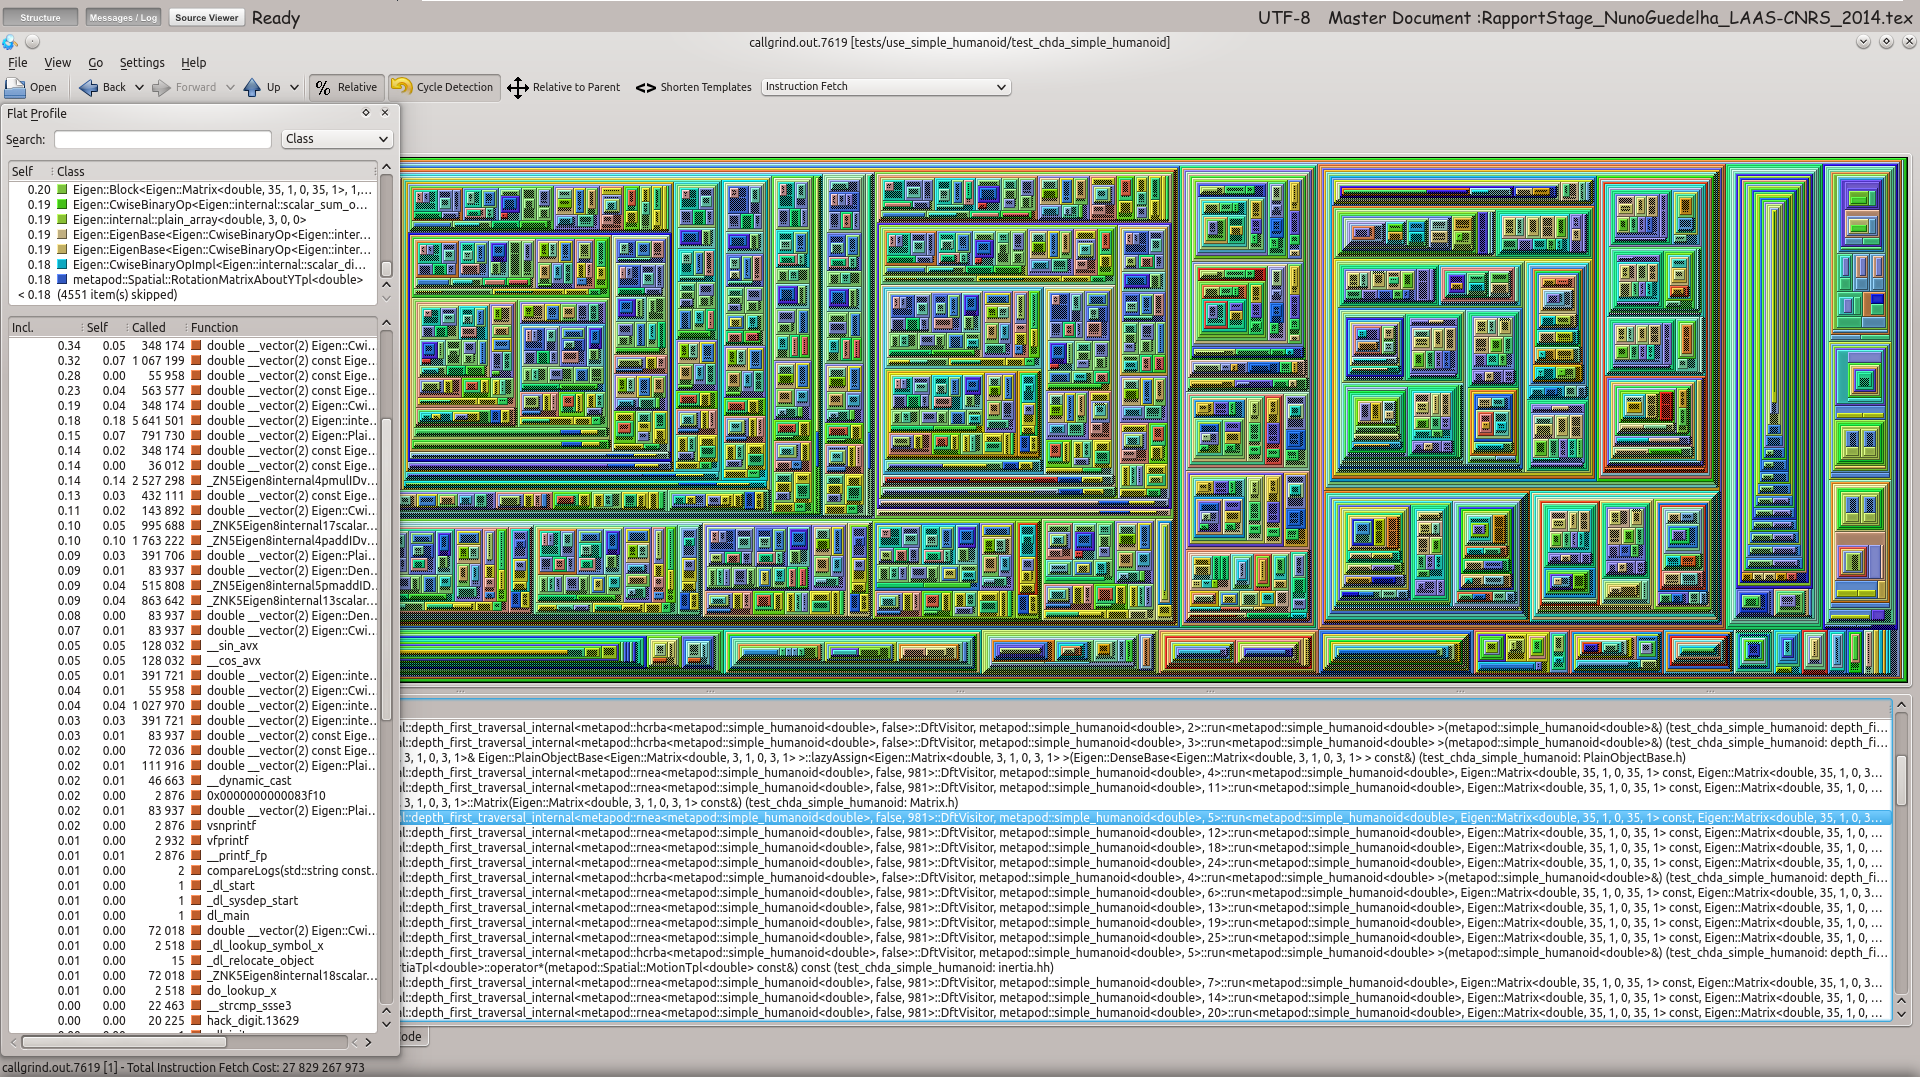
\includegraphics[width=\textwidth]{figs/snapshotKcachegrind1.png}
  \caption{Capture d'écran de Kcachegrind. Visualisation sous Kcachegrind du profil d'exécution des fonctions appelées par $test\_chda$.}         % legende
  \label{fig:Kcachegrind1} % pour citer le numéro de figure
  \end{center}
\end{figure}



\chapter{Concepts et théorèmes en mécanique du solide à la base de l'algèbre spatiale} \label{appx_torseursToalgSpa}

\section{Les torseurs} \label{appx_torseursToalgSpa_torseurs}

\setmyFiguresFile{torseurs}

\subsection{Définition} \label{appx_torseursToalgSpa_torseurs_def}
Les théorèmes généraux de la dynamique des systèmes matériels mettent en jeux deux ensembles de vecteurs liés: celui des quantités de mouvement (cinématique) et celui des forces (dynamique). Ces ensembles n'interviennent que par les torseurs qui leur sont associés. On appelle torseur ($T$) l'ensemble d'un champ antisymétrique $M(A)$ et de son vecteur $S$. $M(A)$ et $S$ sont appelés respectivement \emph{moment} et \emph{vecteur} du torseur $[T]$.

\vspace{0.3cm} % retour à la ligne

\minipages[2]{c}
{.3}{.7}{}
{%
\begin{equation*}
[\underline{T}]=
\begin{bmatrix}
  \underline{S} \\
  \underline{M}(O)
\end{bmatrix}
\end{equation*}
}
{%
\begin{equation}
M(A)=M(B)+AB \times S \textnormal{ ou } M(B)=M(A)+S \times AB
\end{equation}
}
{}

\vspace{0.3cm} % retour à la ligne

Le champ antisymétrique en question n'est pas forcément un champ de vecteurs liés. C'est le cas, par exemple, du torseur cinématique d'un corps rigide en mouvement, constitué à partir du champ antisymétrique des vitesses du solide (vitesse d'un point du solide coïncidant avec un point fixe de l'espace). nous développons ce point dans la section \ref{appx_torseursToalgSpa_torseurs_appl}.

\subsection{Propriétés} \label{appx_torseursToalgSpa_torseurs_prop}

Nous regroupons dans cette section les propriétés des torseurs qui sont directement héritées et utilisées en algèbre spatiale.

\begin{flushleft}
\begin{spacing}{1.5}
\begin{tabular}{ l l c p{5cm} }
  \textbf{\textsc{é}galité:}
  & $[T_{1}]=[T_{2}]$ & $\implies$ & $\mathbf{S}_{1}=\mathbf{S}_{2} \textnormal{ et } \mathbf{M}_{1}(A)=\mathbf{M}_{2}(A)$ \\
  \textbf{Somme:}
  & $[T]=[T_{1}]+[T_{2}]$ & $\implies$ & $\mathbf{S}=\mathbf{S}_{1}+\mathbf{S}_{2} \textnormal{ et } \mathbf{M}(A)=\mathbf{M}_{1}(A)+\mathbf{M}_{2}(A)$ \\
  \textbf{Multiplication par un scalaire:}
  & $[T_{1}]=\lambda [T_{2}]$ & $\implies$ & $\mathbf{S}_{1}=\lambda \mathbf{S}_{2} \textnormal{ et } \mathbf{M}_{1}(A)=\lambda \mathbf{M}_{2}(A)$ \\
  \textbf{Torseur nul:}
  & \multicolumn{3}{l}{$\mathbf{S}=0 \textnormal{ et } \mathbf{M}(A)=0$} \\
  \textbf{Produit scalaire:}
  & $si [F]={\mathbf{F},\mathbf{M}(A)} \textnormal{ et } [v]={\mathbf{w},\mathbf{V}(A)}$ & $\implies$ & $[F][v] = \mathbf{F} \cdot \mathbf{v}(A) + \mathbf{M}(A) \cdot \mathbf{w}$ \\
  \textbf{Invariants:}
  & \multicolumn{3}{l}{(équiprojectivité) la projection de $\mathbf{M}$ sur $\mathbf{S}$} \\
  & \multicolumn{3}{l}{(équiprojectivité) la projection de $\mathbf{M}$ sur $\mathbf{AB}$} \\
  & \multicolumn{3}{l}{Le produit scalaire $[F][v]$.} \\
  \multicolumn{1}{p{6cm}}{\textbf{Torseur lié à un ensemble de vecteurs liés:}}
  & \multicolumn{3}{p{10cm}}{Le moment d'un ensemble de vecteurs liés ${(A_{i},\mathbf{V}_{i})}$ a la forme d'un champ antisymétrique \cite{bib_champVecteurs} (chapitre IV). On lui associe donc
  le torseur} \\
  & \multicolumn{3}{l}{$\mathbf{S}=\Sigma_{i}\mathbf{V}_{i} (\emph{vecteur}) \textnormal{ et } \mathbf{M}(O)=\Sigma_{i}\mathbf{OA}_{i} \times \mathbf{V}_{i} (\emph{moment}).$} \\
\end{tabular}
\end{spacing}
\end{flushleft}

%Fixe la largeur de la 1ere colonne
%\newlength{\my1rstColumnWidth}
%\settowidth{\my1rstColumnWidth}{Multiplication par un scalaire:}
%\setlength{\my1rstColumnWidth}{.5in}

Remarque: on appelle invariants d'un torseur les quantités qui restent constantes quelque soit le point fixe dans l'espace où ce torseur est définit.

\subsection{applications} \label{appx_torseursToalgSpa_torseurs_appl}

\subparagraph{Torseur-vitesse:}

Dans l'étude de la dynamique des systèmes matériels, le champ de vitesses d'un corps rigide en mouvement \footnote{on se limite ici au cas des corps rigides} a la forme d'un champ antisymétrique (vecteurs non liés au corps), et son vecteur $\mathbf{w}$ définit la vitesse angulaire de rotation du solide. On lui associe donc un torseur dont les éléments de réduction sont:

\minipages[2]{|c}
{.75}{.4}{}
{%
\medskip
\begin{description}
  \item[vecteur $\mathbf{S}$:] vitesse angulaire $\mathbf{\omega}$ autour de l'axe de rotation considéré passant par $O$
  \item[moment $\mathbf{M}(O)$:] vitesse linéaire $\mathbf{v}(O)$ du solide au point $O$
\end{description}
\medskip
}{%
\\
\begin{tabular}{|r}
\(
\widehat{\underline{v}}_O=
\begin{bmatrix}
  \mathbf{\underline{S}}    \\
  \mathbf{\underline{M}}(O)
\end{bmatrix}
=
\begin{bmatrix}
  \mathbf{\underline{\omega}} \\
  \mathbf{\underline{v}}_O
\end{bmatrix}
\)
\end{tabular}
\medskip
}
{}

Et on peut exprimer la vitesse de deux points quelconques $A$ et $B$ liés au solide, par rapport à un repère fixe $R$, sous la forme:

\begin{equation}
\mathbf{v}_{B/\emph{R}}=\mathbf{v}_{A/\emph{R}}+\mathbf{BA} \times w_{S/\emph{R}}
\end{equation}
Nous retrouvons ici la forme de la vitesse spatiale établie dans la section \ref{algSpa_Vitesse}.

\subparagraph{Torseur cinétique:}

Le centre de masse $C$ d'un solide quelconque est défini par:
\begin{equation}
\mathbf{OC} = \frac{1}{M} \int_\vartheta \! \mathbf{OA}\rho \mathrm{d} \vartheta
\end{equation}
Où $\rho$ est la masse volumique, $\vartheta$ le volume total du corps rigide et $M$ sa masse totale. La quantité de mouvement $\mathbf{P}$ se calcule en intégrant les quantités de mouvement élémentaires $v \mathrm{d}m$ sur tout le volume $\vartheta$:
\begin{equation}
\mathbf{P} = \int_\vartheta \mathbf{v} \mathrm{d}m = \int_\vartheta \rho \mathbf{v} \mathrm{d}v = M\mathbf{v}_{C}
\end{equation}
De même, le moment cinétique $\mathbf{L}_{O}$ ($O$ origine d'un repère fixe dans l'espace) se calcule en intégrant les moments cinétiques élémentaires sur tout le volume $\vartheta$. Il en résulte une relation simple entre les moments cinétiques en $O$ et un autre point quelconque fixe de $\mathcal{R}$, $O'$:
\begin{equation}\label{momentKantiSym}
\mathbf{L}_O = \int_\vartheta \mathbf{OA} \times \mathbf{v}_A \rho \mathrm{d} \vartheta \quad \textnormal{ et } \quad \mathbf{L}_O = \mathbf{OO'} \times \mathbf{P} + \mathbf{L}_{O'}
\end{equation}
De plus, le théorème de Koenig permet de relier les moments cinétiques $\mathbf{L}_O$ par rapport à $\mathcal{R}$ et $\mathbf{L}^*$ par rapportà  $\mathcal{R^*}$, $\mathcal{R^*}$ étant le repère où le centre de masse est fixe. Le calcul de $\mathbf{L}_O$ dans $\mathcal{R}$ est ainsi simplifié:
\[
\begin{alignedat}{2}
\mathbf{L}_C = \mathbf{L}^* \quad \implies \quad \mathbf{L}_O = \mathbf{OC} \times \mathbf{P} + \mathbf{L}^* \quad \textnormal{ avec } &\quad \mathbf{L}^* &&= \int_\vartheta \rho \mathbf{CA} \times \mathbf{v}^* \mathrm{d} \vartheta \\
\textnormal{(Pour un solide)} &\quad \mathbf{L}^* &&= [I]_C \mathbf{\omega}
\end{alignedat}
\]

\textbf{Remarque:} Dans le cas d'un solide $\mathcal{S}$ en rotation ayant un point fixe $O$ dans $\mathcal{R}$, le moment cinétique exprimé en $O$ est donné par 
\colorbox[gray]{0.8}{\( \mathbf{L}_{O/\mathcal{R}} = [I]_O \mathbf{\omega} \)}, 
où $\mathbf{\omega}$ est le vecteur rotation du solide et $[I]_O$ est l'opérateur d'inertie dans $\mathcal{R}$. Or le centre de masse $C$ de $\mathcal{S}$ est bien un point fixe de $\mathcal{R^*}$, donc on obtient \colorbox[gray]{0.8}{\( \mathbf{L^*} = \mathbf{L}_{C/\mathcal{R^*}} = [I]_C \mathbf{\omega} \)}.

La relation entre les moments cinétiques en deux points fixes $O$ et $O'$ étant antisymétrique \eqref{momentKantiSym}, on peut associer au système de vecteurs liés $\{\rho \mathbf{v}_A \mathrm{d}\vartheta\}$, le torseur $[P]$ dit \emph{torseur cinétique}:

\minipages[2]{|c}
{.6}{.6}{}
{%
\medskip
\begin{description}
\item[moment $\mathbf{M}(O)$:] moment cinétique  $\mathbf{L}_O$ du solide au point $O$
\item[vecteur $\mathbf{S}$:] quantité de mouvement du système $\mathbf{P}$
\end{description}
\medskip
}{%
\\
\begin{tabular}{|r}
\(
\widehat{\underline{P}}_O=
\begin{bmatrix}
  \mathbf{\underline{M}}(O) \\
  \mathbf{\underline{S}}
\end{bmatrix}
=
\begin{bmatrix}
  \mathbf{\underline{\mathbf{L}}}_O \\
  \mathbf{\underline{P}}
\end{bmatrix}
\)
\end{tabular}
\medskip
}
{}


\subparagraph{Torseur-force:}

nous considérons maintenant les forces appliquées au solide $\mathcal{S}_d$ (déformable dans le cas général), toujours en mouvement par rapport au référentiel $\mathcal{R}$. Soit le vecteur lié générique $(A,\mathbf{f}_v)$ représentant la force volumique appliquée à l'élément de matière de volume $\mathrm{d}\vartheta$ qui entoure $A$, un point fixe de $\mathcal{S}$ (figure \ref{fig_systemeDeForces.a}. Cette force inclut les forces extérieures à $\mathcal{S}_d$ ainsi que les forces exercées par les autres éléments de matière de $\mathcal{S}_d$. Notamment, si le référentiel n'est pas galiléen, il faut compter également les forces de Coréolis. On représente donc le système de forces appliquées à $\mathcal{S}_d$ par l'ensemble des vecteurs liés ${(A,\mathbf{f}_v\mathrm{d}\vartheta)}$, pour lequel on calcule la somme des forces et le moment (couple) résultant des forces $O$:

\begin{equation}
\mathbf{f} = \int_\vartheta \mathbf{f}_v\mathrm{d}\vartheta \textnormal{ et } \mathbf{n}_O = \int_\vartheta \mathbf{OA} \times \mathbf{f}_v\mathrm{d}\vartheta
\end{equation}

\dispThreeFig[H]
{1}{vecteur force volumique lié}
{2}{somme des forces et moment des forces}
{3}{Transformation: moment par rapport à un autre point $O'$}
{système de forces des vecteurs liés ${(A,\mathbf{f}_v\mathrm{d}\vartheta)}$}
{fig_systemeDeForces}

Dans cette représentation, on considère $S$ comme une force linéaire globale passant par $O$, avec son moment global $M$ en $O$ associé (figure \ref{fig_systemeDeForces.b}).
On calcule également la relation simple entre les moments des forces en $O$ et un autre point quelconque fixe de $\mathcal{R}$, $O'$ (figure \ref{fig_systemeDeForces.c}):
\begin{equation}\label{}
\mathbf{n}_O = \int_\vartheta (\mathbf{OO'} + \mathbf{O'A}) \times \mathbf{f}_v\mathrm{d}\vartheta = \mathbf{n}_{O'} + \mathbf{OO'} \times \mathbf{f}
\end{equation}

On peut donc associer au système de vecteurs liés ${(A,\mathbf{f}_v\mathrm{d}\vartheta)}$ le torseur $[F]$ dit \emph{torseur-force}:

\minipages[2]{|c}
{.7}{.6}{}
{%
\medskip
\begin{description}
\item[moment $\mathbf{M}(O)$:] couple résultant des forces $\mathbf{n}_O$ du solide au point $O$
\item[vecteur $\mathbf{S}$:] somme des forces du système $\mathbf{f}$
\end{description}
\medskip
}{%
\\
\begin{tabular}{|r}
\(
\widehat{\underline{f}}_O=
\begin{bmatrix}
  \mathbf{\underline{M}}(O) \\
  \mathbf{\underline{S}}
\end{bmatrix}
=
\begin{bmatrix}
  \mathbf{\underline{\mathbf{n}}}_O \\
  \mathbf{\underline{f}}
\end{bmatrix}
\)
\end{tabular}
\medskip
}
{}

Remarque: Les torseurs $\widehat{f}_O$ et $\widehat{f}_O'$ sont équivalents car ils décrivent les mêmes force/mouvement du centre de masse et couple autour du centre de masse du solide. Cette équivalence n'est pas forcément vraie pour l'ensemble du système de forces (par exemple le cas d'un ressort soit comprimé soit étiré par deux forces parallèles et opposées).


\subparagraph{Torseur dynamique:}

Comme pour la quantité de mouvement $P$ et le moment cinétique $L$, nous calculons la quantité d'accélération (somme dynamique) et le moment résultant de cette accélération (moment dynamique) en intégrant les grandeurs élémentaires respectives sur tout le volume, et nous montrons que:
\begin{align}
\mathbf{D} &= \int_\vartheta \mathbf{a} \mathrm{d}m = \frac{\mathrm{d}}{\mathrm{d}t} \int_\vartheta \mathbf{v} \mathrm{d}m = \frac{\mathrm{d}}{\mathrm{d}t} (M \mathbf{v}_{C}) \\
\mathbf{L}_O &= \int_\vartheta \mathbf{OA} \times \rho \mathbf{a}_A \mathrm{d} \vartheta \quad \textnormal{ et } \quad \mathbf{N}_O = \mathbf{OO'} \times \mathbf{D} + \mathbf{N}_{O'}
\end{align}
où $O'$ est un autre point fixe de $\mathcal{R}$.

\medskip

On peut donc associer au système de vecteurs liés ${(A,\rho \mathbf{a}_A \mathrm{d}\vartheta)}$ le torseur $[D]$ dit \emph{torseur dynamique}:

\minipages[2]{|c}
{.7}{.6}{}
{%
\medskip
\begin{description}
\item[moment $\mathbf{M}(O)$:] moment dynamique résultant $\mathbf{N}_O$ du solide au point $O$
\item[vecteur $\mathbf{S}$:] quantité d'accélération du centre de masse $\mathbf{D}$
\end{description}
\medskip
}{%
\\
\begin{tabular}{|r}
\(
\widehat{\underline{D}}_O=
\begin{bmatrix}
  \mathbf{\underline{M}}(O) \\
  \mathbf{\underline{S}}
\end{bmatrix}
=
\begin{bmatrix}
  \mathbf{\underline{\mathbf{N}}}_O \\
  \mathbf{\underline{D}}
\end{bmatrix}
\)
\end{tabular}
\medskip
}
{}



\chapter{Quelques démonstrations en algèbre spatiale} \label{appx_dem}

\setmyFiguresFile{figures}

\section{Invariance du vecteur spacial $\widehat{v}$}

Si on définit deux bases de \emph{Plücker} différentes $D_{O}$ et $D_{P}$, centrées respectivement sur $O$ et $P$:

\begin{align*}
D_{O} = \lbrace &\textbf{d}_{Ox}, \textbf{d}_{Oy}, \textbf{d}_{Oy}, \textbf{d}_{x}, \textbf{d}_{y}, \textbf{d}_{z} \rbrace \\
D_{P} = \lbrace &\textbf{d}_{Px}, \textbf{d}_{Py}, \textbf{d}_{Py}, \textbf{d}_{x}, \textbf{d}_{y}, \textbf{d}_{z} \rbrace \\
\end{align*}

Ainsi que les vecteurs spatiaux associés $\widehat{v}$ et $\widehat{v'}$, on obtient:

\begin{align}
\widehat{v}  &= \underline{v}_{O} \cdot D_{O} \notag \\
\widehat{v'} &= \underline{v}_{P} \cdot D_{P} \notag \\
^{D_{O}}\widehat{v} \quad &= \quad ^{D_{O}}\widehat{v'}
\label{equ_invariant}
\end{align}


Les projections de ces deux vecteurs spatiaux $\widehat{v}$ et $\widehat{v'}$ dans la même base de \emph{Plücker} sont identiques \eqref{equ_invariant}. Il faut noter que si les deux bases ont la même orientation, elles auront les mêmes vecteurs unitaires de translation ($\textbf{d}_{x}$, $\textbf{d}_{y}$ et $\textbf{d}_{z}$), mais les vecteurs unitaires de rotations diffèrent si $O \neq P$ ne sont pas confondus, comme illustré dans le l'exemple de cas simple ci-dessous:

\dispThreeFig[H]
{4}{Deux bases de \emph{Plücker} de même orientation.}
{5}{Expression de $\textbf{d}_{Py}$ et $\textbf{d}_{Pz}$ en $O$.}
{6}{cas de $\textbf{d}_{Pz}$ (projection suivant $\textbf{d}_{z}$).}
{Expression de $\textbf{d}_{Px}$, $\textbf{d}_{Py}$ et $\textbf{d}_{Pz}$ en $O$.}
{vitessePointCoincidant}


Pour rapidement comprendre ces transformations, on peut visualiser un corps tournant autour de l'axe $P_{y}$ à la vitesse $w_{y}$. On définit initialement le vecteur spatial $\widehat{v'}$ en $P$ (\cad considérant l'axe de rotation du corps autour de $P_{y}$) est alors $w_{y}\textbf{d}_{Py}$. Or la vitesse d'un point lié au corps et passant par $O$ (par rapport au repère fixe $R(O,x,y,z)$) vaut $rw_{y}\textbf{d}_{z}$. Le vecteur spatial en $O$ (\cad considérant le corps en rotation autour de l'axe $O_{y}$) est alors $\widehat{v}=\textbf{d}_{Oy}+r\textbf{d}_{z}$. Nous montrons ainsi, pour tous les axes, que:

\begin{align*}
  \textbf{d}_{Px} &= \textbf{d}_{Ox} \\
  \textbf{d}_{Py} &= \textbf{d}_{Oy}+r \textbf{d}_{z} \\
  \textbf{d}_{Pz} &= \textbf{d}_{Oz}-r \textbf{d}_{y}
\end{align*}

On considère à présent un corps $C$ en translation et en rotation autour d'un axe quelconque dans l'espace. Le vecteur spatial $\widehat{v}$ de ce corps en $O$, s'exprime dans la base de \emph{Plücker} $D_{O}$ comme suit:

\begin{equation*}
  \widehat{v} = w_{x}\textbf{d}_{Ox} + w_{y}\textbf{d}_{Oy} + w_{z}\textbf{d}_{Oz} + v_{Ox}\textbf{d}_{x} + v_{Oy}\textbf{d}_{y} + v_{Oz}\textbf{d}_{z}
\end{equation*}

Le vecteur spatial $\widehat{v'}$ de ce corps en $P$, s'exprime dans la base de \emph{Plücker} $D_{P}$ comme suit:

\begin{equation*}
  \widehat{v'} = w_{x}\textbf{d}_{Px} + w_{y}\textbf{d}_{Py} + w_{z}\textbf{d}_{Pz} + v_{Px}\textbf{d}_{x} + v_{Py}\textbf{d}_{y} + v_{Pz}\textbf{d}_{z}
\end{equation*}

Nous voulons l'exprimer dans la base $D_{O}$. $w_{x}$, $w_{y}$ et $w_{z}$ sont connus. Calculons $v_{Px}$, $v_{Py}$ et $v_{Pz}$:

\vspace{0.3cm}
\minipages[2]{t}{.4}{.6}{}
{%
\(
\begin{alignedat}{3}
  & &&\phantom{xxx} v_{P} &&= v_{O} + w \times \overrightarrow{OP} \\
  \vspace{0.5cm}
  &\iff &&\phantom{xxx} \underline{v}_{P}
  &&=
  \underline{v}_{O}+\underline{w}\times
  \begin{bmatrix}
    r\\
    0\\
    0
  \end{bmatrix} \\
  \vspace{0.5cm}
  &\iff
  &&\begin{bmatrix}
    v_{Px} \\
    v_{Py} \\
    v_{Pz}
  \end{bmatrix}
  &&=
  \begin{bmatrix}
    v_{Ox}\\
    v_{Oy}+w_{z}r\\
    v_{Oz}-w_{y}r
  \end{bmatrix}
  \quad \texttt{or} \quad
  \widehat{\underline{v}'}
  =
  \begin{bmatrix}
    \underline{w} \\
    \underline{v}_{P}
  \end{bmatrix}
\end{alignedat}
\)}
{%
\begin{tabular}{|p{\textwidth}}
\(\begin{alignedat}{2}
  &\iff
  \widehat{v'} &&= w_{x}\textbf{d}_{Px} + w_{y}\textbf{d}_{Py} + w_{z}\textbf{d}_{Pz} \\
  &            &&\phantom{{}={}} + v_{Px}\textbf{d}_{x} + v_{Py}\textbf{d}_{y} + v_{Pz}\textbf{d}_{z} \\
  &            &&= w_{x}\textbf{d}_{Ox} + w_{y}(\textbf{d}_{Oy}+r\textbf{d}_{z}) + w_{z}(\textbf{d}_{Oz}-r\textbf{d}_{y}) \\
  &            &&\phantom{{}={}} + v_{Ox}\textbf{d}_{x} + (v_{Oy}+w_{z}r)\textbf{d}_{y} + (v_{Oz}-w_{y}r)\textbf{d}_{z} \\
  &            &&= w_{x}\textbf{d}_{Ox} + w_{y}\textbf{d}_{Oy} + w_{z}\textbf{d}_{Oz} + v_{Ox}\textbf{d}_{x} + v_{Oy}\textbf{d}_{y} + v_{Oz}\textbf{d}_{z} \\
  &            &&= \widehat{v}
\end{alignedat}\)
\end{tabular}
}
{}
\vspace{0.3cm}

Nous avons ainsi montré l'équivalence des deux vecturs spatiaux $\widehat{v}$ et $\widehat{v'}$.

La propriété d'invariance se vérifie pour tout point $O$ et $P$ fixes dans l'espace et une orientation quelconque des repères $R(O,x,y,z)$ et $R'(P,x,y,z)$. Nous pouvons trouver la démonstration complète de cette propriété d'invariance dans l'annexe \ref{appx_dem}.










% Bibliography:
\clearpage
\addcontentsline{toc}{chapter}{Bibliography}

\begin{thebibliography}{9}

\bibitem{bib_featherstone}
  Roy Featherstone,
  \emph{Rigid Body Dynamics Algorithms}.
  Springer Science+Business Media, LLC,
  $2^{nd}$ edition,
  2008.

\bibitem{bib_torseur}
  E. Ramis, C. Deschamps et J. Odoux,
  \emph{Algèbre et applications à la géométrie}.
  Masson, coll. "Cours de mathématiques spéciales"
  $2^{edition}$, 1987 (ISBN 2-225-63404-1),
  chap. 8 ("Les torseurs"), p. 276-294
  
\bibitem{bib_champVecteurs}
  José-Philippe Pérez,
  \emph{Mécanique, Fondements et applications}.
  Masson Sciences,
  $6^{e}$ édition, 2001 (ISBN 2-10-005464-3),
  chap. 1 ("Calcul vectoriel. Torseurs") - section IV, V et VI - p. 8-15, 
  chap. 16 (Cinématique du solide et des solides en contact) - section I - p. 257, 295
  
\bibitem{bib_eigen_tutorial_alg_lin}
  Eigen - Tutorial Linear Algebra:
  http://eigen.tuxfamily.org/dox/%group__TutorialLinearAlgebra.html
  
\bibitem{bib_eigen_tutorial_catalogue}
  Eigen - Catalogue of dense decompositions,
  %http://eigen.tuxfamily.org/dox/group__TopicLinearAlgebraDecompositions.html
  
\bibitem{bib_eigen_LLT_desc}
  Eigen - LLT detailed description,
  %http://eigen.tuxfamily.org/dox/classEigen_1_1LLT.html

\bibitem{bib_eigen_tutorial_catalogue_sparse}
  Eigen - Solving Sparse Linear Systems
  %http://eigen.tuxfamily.org/dox/group__TopicSparseSystems.html

\bibitem{bib_ros}
  ROS - site internet:
  http://wiki.ros.org/urdf/

\bibitem{bib_urdf}
  URDF - page internet sous le site ROS:
  http://wiki.ros.org/urdf/

%\bibitem{bib_matriceDefiniePositive_1}
%Horn & Johnson (1985), p. 397

%\bibitem{bib_matriceDefiniePositive_2}
%http://en.wikipedia.org/wiki/Positive-definite_matrix

%\bibitem{bib_openMPcompilers}
%  "OpenMP Compilers"at OpenMP.org,
%  http://openmp.org/wp/openmp-compilers/
%  2013-04-10. Retrieved 2013-08-14.

\bibitem{bib_openMPspecs}
  The OpenMP API specification for parallel programming,
  http://openmp.org/wp/openmp-specifications/

\bibitem{bib_openMpWikipedia}
  http://en.wikipedia.org/wiki/OpenMP
  
\bibitem{bib_decompositionLUwikipedia}
  Wikipedia% - Décomposition LU
%  http://fr.wikipedia.org/wiki/Décomposition_LU

\bibitem{bib_decompositionLU_1}
  Cours d'analyse numérique de licence (2010) de R. Herbin, Université d'Aix-Marseille, section 1.3.1, pages 25-26
  http://www.cmi.univ-mrs.fr/~herbin/PUBLI/anamat.pdf
  
\bibitem{bib_decompositionLU_2}
  P. G. Ciarlet - « Introduction à l'analyse numérique matricielle et à l'optimisation » (1985, rééd. 2001), éd. Masson, coll. Math. Appl. pour la Maîtrise (ISBN 2-225-68893-1)

%\bibitem{bib_complexiteInversionMatriceDirecte}
%  SUR L'INVERSION DE MATRICE,
  J.B Lasserre,
%  http://archive.numdam.org/ARCHIVE/RO/RO_1992__26_2/RO_1992__26_2_177_0/RO_1992__26_2_177_0.pdf

\end{thebibliography}



\end{document}
